\title{Neural Networks - Project: Part A}
\author{Ryan Spangler}
\date{\today}

\documentclass[12pt]{article}

\usepackage{commath}
\usepackage{graphicx}
\usepackage{listings}
\usepackage{amsfonts}

% python highlighting ----------
\usepackage{color}
\usepackage{listings}
\usepackage{textcomp}
\usepackage{setspace}
%\usepackage{palatino}

\renewcommand{\lstlistlistingname}{Code Listings}
\renewcommand{\lstlistingname}{Code Listing}
\definecolor{gray}{gray}{0.6}
\definecolor{green}{rgb}{0.1,0.6,0.3}
\definecolor{orange}{rgb}{0.9,0.7,0.1}
\definecolor{blue}{rgb}{0,0.6,0.8}

\lstnewenvironment{python}[1][]{
\lstset{
language=python,
basicstyle=\ttfamily\footnotesize\setstretch{1},
stringstyle=\color{red},
showstringspaces=false,
alsoletter={1234567890},
otherkeywords={\ , \}, \{},
keywordstyle=\color{blue},
emph={access,and,break,class,continue,def,del,elif,else,%
except,exec,finally,for,from,global,if,import,in,is,%
lambda,not,or,pass,print,raise,return,try,while},
emphstyle=\color{gray}\bfseries,
emph={[2]True, False, None, self},
emphstyle=[2]\color{orange},
emph={[3]from, import, as},
emphstyle=[3]\color{blue},
upquote=true,
morecomment=[s]{"""}{"""},
commentstyle=\color{gray}\slshape,
emph={[4]1, 2, 3, 4, 5, 6, 7, 8, 9, 0},
emphstyle=[4]\color{blue},
literate=*{:}{{\textcolor{blue}:}}{1}%
	{=}{{\textcolor{blue}=}}{1}%
	{-}{{\textcolor{blue}-}}{1}%
	{+}{{\textcolor{blue}+}}{1}%
	{*}{{\textcolor{blue}*}}{1}%
	{!}{{\textcolor{blue}!}}{1}%
	{(}{{\textcolor{blue}(}}{1}%
	{)}{{\textcolor{blue})}}{1}%
	{[}{{\textcolor{blue}[}}{1}%
	{]}{{\textcolor{blue}]}}{1}%
	{<}{{\textcolor{blue}<}}{1}%
	{>}{{\textcolor{blue}>}}{1},%
    frame=fullbox, rulesepcolor=\color{gray},#1
%framexleftmargin=1mm, framextopmargin=1mm, frame=shadowbox, rulesepcolor=\color{blue},#1
}}{}

\setcounter{secnumdepth}{0}

\begin{document}
\maketitle

\section{Familiarization with Land-Use Data}

\subsection{Problem Statement}

The purpose of this phase of the project was to become familiar with the land-use data from 1974, and use the data to train a backpropagation network under various experimental conditions.  Once the networks are trained, find a way to evaluate the effectiveness of the training on this data by plotting the performance over the training period for each experimental approach relative to one another.

\subsection{Experimental Process}

The results I was looking for were the percentages of correct matches over the training process for each set of parameters given to the network.  In order to obtain results for this data set a number of steps were necessary:

\begin{enumerate}
\item Train the network on the training set for 2000 cycles.
\item Take a snapshot of the network.
\item Repeat training process until 30000 cycles have been reached.
\item Go through all the snapshots and test the performance using both recall and generalization of unseen i/o pairs, outputting the results to a .nnr file.
\item Parse and analyze the each set of .nnr files for each set of network parameters, identifying correct matches for each one.
\item Plot all of the learning curves for each network, so that their performance can be compared relative to one another.
\end{enumerate}

For the last two items I wrote a python program using python's numerical matrix and plotting libraries provided by pylab.  

Besides the control trial which ran with default parameters, the five parameters that varied during the trials were:

\begin{itemize}
\item Setting the momentum to 0.2 (from 0.4).
\item Setting the epoch to 64 rather than 16.
\item Upping the learning coefficient from 0.5 to 0.75.
\item Using the quickprop learning algorithm rather than the usual delta rule.
\item Using a sine transfer function rather than a sigmoid.  (I knew this would probably not perform well, I just wanted to see the effect it would have and if it could learn anything at all based on a sine transfer).
\end{itemize}

\subsection{Results}

This hard-won graph sums up the results of the trials.  When the momentum was 0.2 rather than 0.4, it took longer to get to the asymptotic limit of about 90\% correct matches.  Upping the learning coefficient to 0.75 ultimately led to better results than the lower value of 0.5, but not by much.  The quickprop learning algorithm performed badly, having a spike towards the end but never really even reaching 50\%.  Changing the epoch to 64 did not change the results at all, they were identical to the control.  The sine transfer function after a modest spike settled at around 20\% effectiveness.  

\begin{figure}[h!]
  \centering
    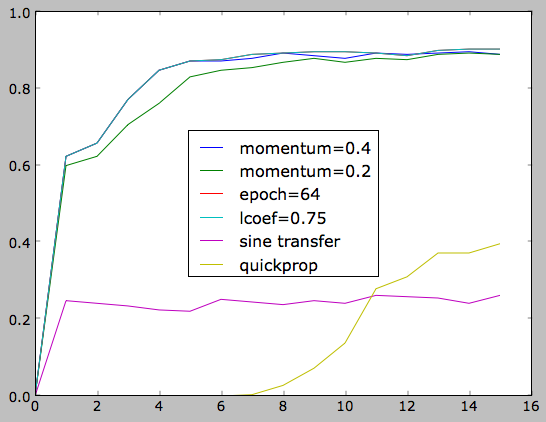
\includegraphics[scale=0.6]{results.png}
  \caption{In the above graph the x-axis is over the number of checkpoints and the y-axis is the percentage of correct guesses.  There were 15 checkpoints in all over trials of 30000 cycles each.}
\end{figure}

Here is the python code used to analyze the results and generate the graphs:

\begin{python}[]

from pylab import *

def suffix(n):
    s = str(n)
    p = '0' * (3-len(s))
    return p + s

class NNR:
    def __init__(self, filename):
        self.filename = filename

        contents = open(filename).read()
        lines = contents.split("\n")
        lines.pop()

        self.data = array(
            map(lambda line: map(
                    lambda x: float(x), line.split("\t")[1:]), 
                lines))

        self.outputs = self.data.shape[1] / 2
        self.expected = self.data[:,:self.outputs]
        self.results = self.data[:,self.outputs:]
        self.diff = self.expected - self.results
        self.mask = self.expected * self.results

        self.strict = map(
            lambda p: all(map(
                lambda x: abs(x) < 0.2, p)), self.diff)
        self.loose = map(
            lambda p: abs(sum(p) - 1.0) < 0.2, self.mask)
        self.error = sum(self.diff)

    def performance(self):
        return float(sum(self.loose)) / float(len(self.loose))

class Series:
    def __init__(self, base, steps, desc):
        self.base = base
        self.steps = steps
        self.desc = desc

        self.nnr = map(lambda x: NNR(base+suffix(x)), range(steps))
        self.data = array(map(lambda d: d.performance(), self.nnr))

    def plot(self):
        plot(self.data, label=self.desc)

class Experiment:
    def __init__(self, series, steps):
        self.series = map(
            lambda s: Series('phtrain/'+s[0], steps, s[1]), series)
        
    def plot(self):
        for s in self.series:
            s.plot()
        legend(loc='middle right')

def run():
    experiment = Experiment([
      ('fourmom', 'momentum=0.4'), 
      ('twomom', 'momentum=0.2'),
      ('epoch64', 'epoch=64'),
      ('highlcoef', 'lcoef=0.75'),
      ('sine', 'sine transfer'),
      ('quickprop', 'quickprop')], 16)

    experiment.plot()
    return experiment

\end{python}

\end{document}  

